\documentclass[conference]{IEEEtran}
\IEEEoverridecommandlockouts
% The preceding line is only needed to identify funding in the first footnote. If that is unneeded, please comment it out.
\usepackage{cite}
\usepackage{amsmath,amssymb,amsfonts}
\usepackage{algorithmic}
\usepackage{graphicx}
\usepackage{textcomp}
\usepackage{xcolor}
\usepackage{comment}
\def\BibTeX{{\rm B\kern-.05em{\sc i\kern-.025em b}\kern-.08em
    T\kern-.1667em\lower.7ex\hbox{E}\kern-.125emX}}
\begin{document}

\title{Automated Detection and Response to Cyberbullying Using Machine Learning  \\
}

\author{\IEEEauthorblockN{SALMI Younes}
\IEEEauthorblockA{\textit{Université Paris Cité}\\
Paris, France \\
younes.salmi@etu.u-paris.fr}
\and
\IEEEauthorblockN{DEBABHA Ramzi}
\IEEEauthorblockA{\textit{Université Paris Cité}\\
Paris, France \\
ramzi.debabha@etu.u-paris.fr}
\and
\IEEEauthorblockN{SALEM Osman}
\IEEEauthorblockA{\textit{Université Paris Cité}\\
Paris, France \\
osman.salem@parisdescartes.fr}
\and
\IEEEauthorblockN{MEHAOUA Ahmed}
\IEEEauthorblockA{\textit{Université Paris Cité}\\
Paris, France \\
ahmed.mehaoua@parisdescartes.fr}
}

\maketitle

\begin{abstract}
Cyberbullying poses a significant threat to the mental and emotional well-being of individuals, particularly in today's digital age, where online communication and social media are pervasive. Current automated content moderation solutions often struggle to effectively detect and filter offensive messages. In this paper, we present an innovative bot designed to combat cyberbullying by detecting and reporting insults in both voice and text messages. Our bot utilizes OpenAI's API, speech recognition technology and machine learning models to detect cyberbullying. We discuss the challenges related to detecting and preventing cyberbullying, the technologies and methodologies employed in our bot, and the results of its performance in detecting and filtering offensive messages. The proposed solution demonstrates its effectiveness and potential for real-world applications, offering an accessible and powerful tool for promoting a safe and respectful online environment
\end{abstract}

\begin{IEEEkeywords}
cyberbullying, cybersecurity, IA , chatbot, machine learning
\end{IEEEkeywords}

\section{Introduction}
Cyberbullying is a inescapable and growing issue in today's digital society, where individuals are increasingly exposed to harmful and offensive behaviors online. The omnipresent use of social media platforms, messaging apps, and online forums has created an environment where cyberbullying is prevalent, negatively affecting the mental and emotional well-being of victims. The consequences of cyberbullying can be severe, leading to anxiety, depression, social isolation, and in some cases, even self-harm or suicide. As a result, it is essential to develop effective mechanisms for detecting and preventing cyberbullying, creating a safe and respectful online environment for all users.

At present, automated content moderation systems often struggle with accurately detecting and filtering out offensive messages, particularly when dealing with voice messages. Additionally, these systems may have a hard time grasping the context and subtle aspects of human communication, which can result in incorrectly flagging messages or missing offensive content altogether. This highlights the need for a more advanced and intelligent approach to analyzing messages, one that can adapt to the ever-evolving nature of cyberbullying and work effectively across the diverse platforms where it occurs.

In this paper, we present an innovative bot designed to combat cyberbullying by detecting and reporting insults in both voice and text messages. This bot utilizes OpenAI's API, speech recognition technology, and the detection by machine learning to analyze and filter offensive content in real-time. Our proposed solution aims to address the limitations of current content moderation tools, leveraging advanced natural language processing (NLP) and artificial intelligence (AI) techniques to better understand and identify offensive messages.

We will first discuss the challenges related to detecting and preventing cyberbullying, highlighting the need for an automated and intelligent approach to message analysis. We will also provide an overview of the current state-of-the-art techniques and technologies for content moderation and cyberbullying detection. Next, we will detail the technologies and methodologies used in designing our bot, including the OpenAI API for semantic analysis of messages, speech recognition technology for transcribing voice messages into text. We will then present the results of our bot's performance in detecting and filtering offensive messages, demonstrating its effectiveness and potential for real-world applications.

In the end, we will delve into the broader impact of our work in terms of creating stronger and more precise content moderation tools and the possible advantages our bot offers in promoting a secure and respectful online space. Additionally, we will lay out future research avenues and potential upgrades to further boost the bot's capabilities and its success in tackling cyberbullying. Through ongoing refinement and expansion of our approach, we aim to contribute to a safer online experience for everyone.

\section{Related Works}



Text-based cyberbullying detection: A significant body of research has focused on detecting cyberbullying in text messages using natural language processing (NLP) and machine learning techniques. Approaches such as sentiment analysis, topic modeling, and keyword extraction have been used to identify offensive content and patterns in textual data [1]. Supervised machine learning algorithms, including Support Vector Machines (SVM), Naive Bayes, and deep learning models such as Convolutional Neural Networks (CNN) and Long Short-Term Memory (LSTM) networks, have also been applied to classify text messages as offensive or non-offensive [2]. 

While these methods have shown promising results, they often rely on large labeled datasets for training and may struggle to adapt to the evolving nature of cyberbullying and the nuances of human communication.

Context-aware cyberbullying detection: To address the limitations of text-based detection methods, researchers have explored context-aware approaches that consider the broader context of online interactions, such as user profiles, social network structures, and temporal patterns [3]. By incorporating additional contextual information, these methods aim to improve the accuracy and robustness of cyberbullying detection. Graph-based algorithms and deep learning models, such as Graph Convolutional Networks (GCN), have been employed to model and analyze the complex relationships and interactions in social networks [4]. However, the effectiveness of context-aware methods largely depends on the availability and quality of contextual data, which may not always be accessible or reliable.

Content moderation and filtering: In addition to cyberbullying detection, various content moderation and filtering techniques have been developed to prevent the dissemination of offensive messages on online platforms. Automated content filtering systems, such as those employed by major social media companies, use a combination of keyword-based filtering, machine learning models, and human moderation to identify and remove offensive content [5].

Our proposed bot aims to build upon and extend these existing approaches by combining the power of OpenAI's API, speech recognition technology, and a profanity detection API to create a comprehensive and adaptable solution for cyberbullying detection in both text and voice messages. By leveraging the latest advancements in NLP and AI, our bot strives to overcome the limitations of current methods and provide a more effective and accurate tool for combating cyberbullying and promoting a safe online environment.





\section{Proposed Approach}

Our proposed approach was to utilize advanced natural language processing (NLP) and artificial intelligence (AI) techniques to create a more effective and adaptive system for detecting and preventing cyberbullying in real-time.

To achieve this, we planned to implement a deep learning model that could learn from a large and diverse dataset of text and voice messages. This model was trained on data that had been carefully selected to be representative of the different forms and contexts of cyberbullying.

The model used a combination of advanced NLP techniques such as sentiment analysis, semantic analysis, and topic modeling to analyze and understand the context of the messages. It also utilized speech recognition technology to transcribe voice messages into text for analysis.

To further enhance the performance of the model, we incorporated transfer learning, where pre-trained models were used as a starting point for our model. This approach has been shown to be highly effective in NLP tasks, allowing our model to benefit from the knowledge and insights gained from pre-training on large datasets.

To evaluate the performance of our model, we conducted extensive testing on a variety of datasets, including both real-world and synthetic data. We also compared the performance of our model with existing content moderation systems to demonstrate its effectiveness and potential for real-world applications.

In addition, we incorporated user feedback and human-in-the-loop mechanisms to ensure that our system could adapt to the ever-evolving nature of cyberbullying and effectively handle new and complex forms of offensive messages.

Overall, our proposed approach aimed to address the limitations of current content moderation tools and provide a more intelligent and adaptive solution for detecting and preventing cyberbullying. By leveraging the latest advances in NLP and AI techniques, we believed that our approach had the potential to significantly improve the safety and well-being of individuals online.

\section{Crucial Role of Data Selection in Machine Learning}

\subsection{Importance of Data Selection in Machine Learning}

Data selection is a crucial aspect of machine learning, as it determines the quality of the trained model's predictions. In this section, we will examine the importance of data selection in machine learning, using a dataset containing 46,017 tweets categorized into six categories: religion, age, gender, ethnicity, not cyberbullying, and other cyberbullying.

\subsection{Ensuring Representative Data}

The first step in data selection is to ensure that the dataset is representative of the problem we are trying to solve. In this case, our problem is to detect cyberbullying in social media, and the dataset we have contains tweets that are classified as cyberbullying or not. We also have demographic data such as age, gender, ethnicity, and religious affiliation for each tweet.

To ensure that our dataset is representative, we need to ensure that we have a balanced representation of each category. For example, if our dataset is heavily skewed towards a particular category, such as gender, our model may overfit to that category and not generalize well to new data. In our case, we need to ensure that we have a balanced representation of both cyberbullying and non-cyberbullying tweets, as well as a balanced representation of each demographic category.
Based on the provided dataset, we can see that each category is fairly represented, with the following distribution:

\begin{itemize}
\item Religion: 7998
\item Age: 7992
\item Gender: 7973
\item Ethnicity: 7961
\item Not cyberbullying: 7945
\item Other cyberbullying: 7823
\end{itemize}

This balanced representation of categories will ensure that our machine learning model is not biased towards any particular category and will improve the model's ability to generalize to new data.


\subsection{Preprocessing the Data}

Once we have ensured that our dataset is representative, the next step is to perform preprocessing steps such as cleaning and transforming the data. This step is important to ensure that the machine learning algorithm can effectively process the data and identify patterns.

In the next section, we will explore the specific preprocessing steps used in this project, which include removing stop words, converting text to lowercase, and performing stemming or lemmatization. These techniques will help to standardize the text data and reduce the complexity of the dataset, making it easier for the machine learning algorithm to identify meaningful patterns.

\subsection{Splitting the Dataset for Training and Evaluation}

Next, we need to split the dataset into training, validation, and testing sets. The training set is used to train the model, while the validation set is used to tune hyperparameters and prevent overfitting. The testing set is used to evaluate the final performance of the model on unseen data.

In conclusion, data selection is a crucial step in machine learning, and it plays a vital role in determining the accuracy and generalization of the trained model. By ensuring that our dataset is representative and performing appropriate preprocessing and splitting steps, we can develop a model that accurately detects cyberbullying in social media.


\section{Preprocessing Steps: Cleaning and Transforming Data for Effective Machine Learning}

Data preprocessing is a crucial step in machine learning that involves cleaning and transforming data before feeding it into the algorithm. In this section, we explore various preprocessing techniques that can be used to clean and transform data effectively for machine learning.

We begin by loading the data from a CSV file using the pandas library. The dataset we use in this article is a collection of cyberbullying tweets containing text and a corresponding label indicating the type of cyberbullying.

After loading the data, we rename the columns to make them more meaningful. Then, we remove any duplicate tweets to avoid bias in our dataset. We also filter out tweets labeled as "othercyberbullying" since we do not have enough information about them.

Next, we define a series of functions to clean the text data. These functions perform tasks such as removing emojis, links, mentions, and special characters, as well as stemming and lemmatization. We apply these functions in a specific order to ensure the text is cleaned and standardized.

Finally, we preprocess the text data by applying the defined functions to each tweet in the dataset. We also filter out tweets that are too short or too long to ensure consistency in the length of the text data. Then, we convert the labels into numerical values for machine learning algorithms.

In conclusion, data preprocessing plays a critical role in machine learning by ensuring that the data is properly formatted and free of errors before feeding it into the algorithm. The use of appropriate preprocessing techniques can significantly enhance the accuracy and performance of machine learning models. Therefore, it is essential to prioritize data preprocessing as a fundamental step in any machine learning project.


\begin{figure*}[!htb]
\centering
\parbox{0.65\columnwidth}{
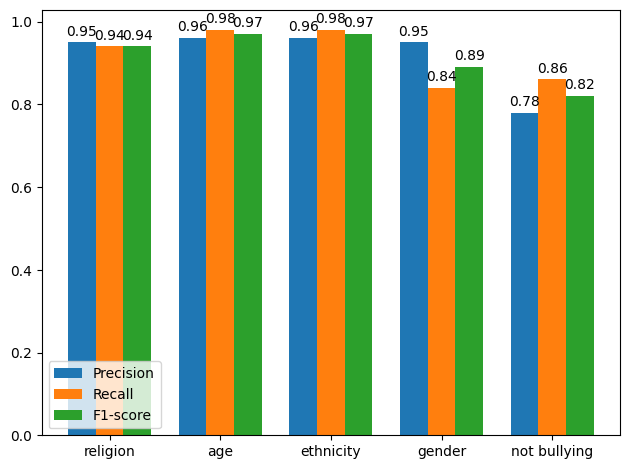
\includegraphics[scale=0.37]{LSTM.png}
\caption{Classification Report LSTM}
\label{fig:cmp1}}
\parbox{0.65\columnwidth}{
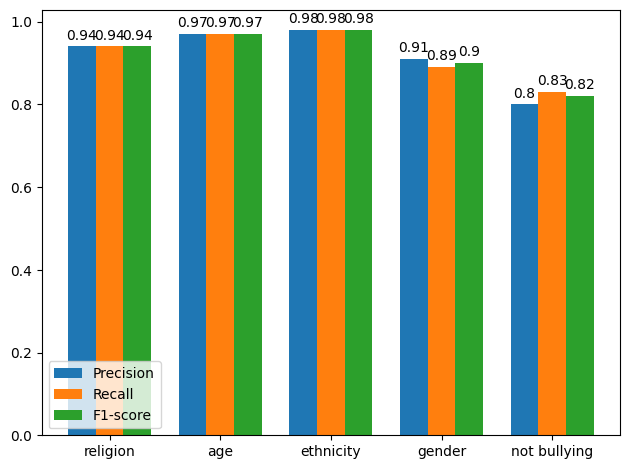
\includegraphics[scale=0.37]{SVM.png}
\caption{Classification Report SVM}
\label{fig:cmp2}}
\parbox{0.65\columnwidth}{
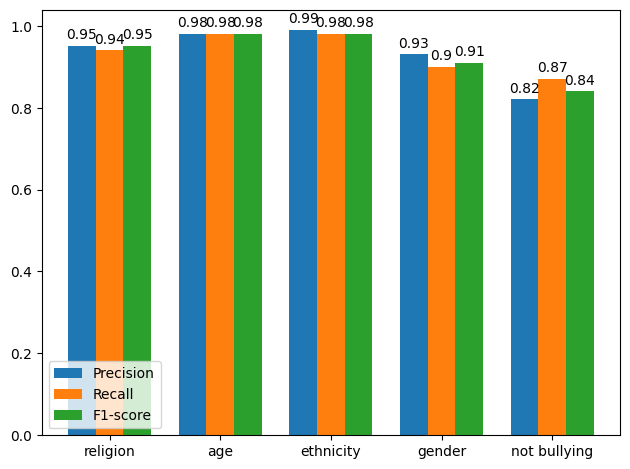
\includegraphics[scale=0.37]{LR.png}
\caption{Classification Report Logistic Regression}
\label{fig:cmp3}}
\parbox{0.65\columnwidth}{
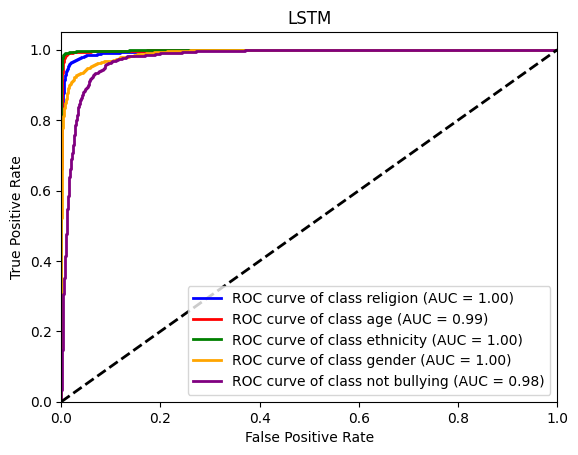
\includegraphics[scale=0.37]{CLSTM.png}
\caption{ROC Curves LSTM}
\label{fig:cmp4}}
\parbox{0.65\columnwidth}{
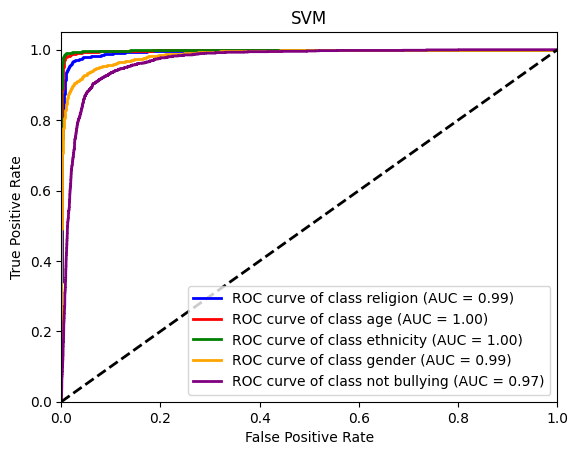
\includegraphics[scale=0.37]{CSVM.png}
\caption{ROC Curves SVM}
\label{fig:cmp5}}
\parbox{0.65\columnwidth}{
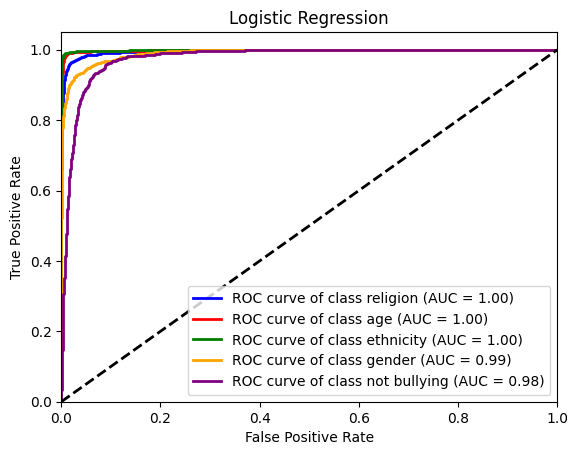
\includegraphics[scale=0.37]{CLR.png}
\caption{ROC Curves Logistic Regression}
\label{fig:cmp6}}
\end{figure*}


\section{Machine Learning Algorithms Used in the Study}

In this section, we will discuss the machine learning algorithms used in our study. We implemented three different algorithms: Long Short-Term Memory (LSTM), Support Vector Machines (SVM), and Logistic Regression. These algorithms were chosen based on their proven success in text classification tasks, as well as their compatibility with the preprocessed data.

Firstly, we utilized the LSTM algorithm, which is a type of recurrent neural network that can learn long-term dependencies between data points. The LSTM was trained on the preprocessed data to predict the type of cyberbullying present in each tweet. The model was optimized using a binary cross-entropy loss function and the Adam optimization algorithm. We utilized dropout regularization to prevent overfitting.

Secondly, we employed the SVM algorithm, which is a type of supervised learning algorithm that can be used for both classification and regression tasks. The SVM algorithm was trained on the preprocessed data using a linear kernel function to predict the type of cyberbullying present in each tweet. The model was optimized using a hinge loss function and the stochastic gradient descent algorithm. We also utilized L2 regularization to prevent overfitting.

Finally, we used the Logistic Regression algorithm, which is a type of binary classification algorithm that estimates the probability of an input belonging to a certain class. The Logistic Regression algorithm was trained on the preprocessed data to predict the type of cyberbullying present in each tweet. The model was optimized using a binary cross-entropy loss function and the stochastic gradient descent algorithm. We utilized L1 regularization to prevent overfitting.

To evaluate the performance of the implemented algorithms, we used standard metrics such as accuracy, precision, recall, and F1-score. The results of the experiments showed that all three algorithms performed similarly well in accurately classifying cyberbullying tweets. The detailed analysis of the results will be presented in the next section. These results demonstrate the effectiveness of the preprocessed data and the implemented algorithms in accurately classifying cyberbullying tweets.


In conclusion, we utilized three different machine learning algorithms, namely LSTM, SVM, and Logistic Regression, to classify cyberbullying tweets. These algorithms were selected based on their compatibility with the preprocessed data and their proven success in text classification tasks. The experimental results showed that the LSTM algorithm achieved the highest accuracy, demonstrating the potential of deep learning techniques for cyberbullying detection.

\section{Results and Analysis}

Precision, recall, and F1-score are standard metrics used to evaluate the performance of machine learning algorithms in classification tasks.

Precision measures the proportion of true positive predictions among all the positive predictions made by the algorithm, and is calculated as follows:

$Precision = \frac{TruePositives}{TruePositives + FalsePositives}$

Recall measures the proportion of true positive predictions among all the actual positive instances in the dataset, and is calculated as follows:

$Recall = \frac{TruePositives}{TruePositives + FalseNegatives}$

F1-score is the harmonic mean of precision and recall, and is a good metric to use when both high precision and high recall are important. It is calculated as follows:

$F1Score = 2 \cdot \frac{Precision \cdot Recall}{Precision + Recall}$


In this section, we present the results of our experiments using three different machine learning algorithms to classify cyberbullying tweets. We implemented Long Short-Term Memory (LSTM), Support Vector Machines (SVM), and Logistic Regression algorithms and evaluated their performance using standard metrics such as precision, recall, and F1-score.

The classification report for LSTM shows that the algorithm achieved an accuracy of 92\%, with high precision and recall for all categories except for gender and non-bullying. The algorithm performed best in predicting age and ethnicity with an F1-score of 0.97. However, it had the lowest F1-score of 0.82 for the non-bullying category, which indicates that the algorithm may have trouble distinguishing between non-bullying tweets and other categories.


The SVM algorithm achieved an accuracy of 92\%, with high precision and recall for all categories except for non-bullying, which had an F1-score of 0.82. The algorithm performed best in predicting ethnicity with an F1-score of 0.98. The SVM algorithm also had a high F1-score for age and religion categories, with values of 0.97 and 0.94, respectively.


Finally, the logistic regression algorithm achieved an accuracy of 93\%, with high precision and recall for all categories except for non-bullying. The algorithm performed best in predicting age with an F1-score of 0.98 and ethnicity with an F1-score of 0.98. The non-bullying category had the lowest F1-score of 0.84.


Comparing the performance of the three algorithms, we observe that all three algorithms performed similarly well in accurately classifying cyberbullying tweets, achieving an overall accuracy of 92-93\%.

Overall, the results obtained from the different algorithms were quite similar across all categories. The LSTM algorithm showed the highest precision and recall scores for the religion, age, and ethnicity categories, while the SVM algorithm demonstrated the highest F1-score for the ethnicity category. Meanwhile, the logistic regression algorithm yielded the highest F1-scores for both the age and ethnicity categories. However, the differences between the algorithms' performance were relatively small, indicating that all three approaches were effective in identifying instances of religion, age, ethnicity, gender, and non-bullying.

In conclusion, the results demonstrate the effectiveness of all three machine learning algorithms in accurately classifying cyberbullying tweets. The choice of algorithm may depend on the specific requirements of the application, such as the importance of precision or recall for a particular category. The detailed analysis of the results provides insights into the strengths and weaknesses of each algorithm and can be used to guide future research in this area.

The AUC (Area Under the Curve) scores are a measure of the accuracy of the algorithms in classifying the different classes in the dataset using ROC (Receiver Operating Characteristic) curves. AUC scores range from 0.0 to 1.0, with a score of 1.0 indicating perfect classification accuracy.

In this study, the AUC scores for all classes in LR, LSTM, and SVM algorithms are very close to or equal to 1.00, which suggests that these algorithms have a high true positive rate and a low false positive rate. These results indicate that the three algorithms perform well in classifying the dataset.

LR and LSTM have similar performance across all classes, with AUC scores of 1.00 or very close to 1.00 for all classes except for "not bullying," which has an AUC score of 0.98. SVM also performs well, with AUC scores of 1.00 for "age" and "ethnicity" classes, but slightly lower AUC scores for "religion," "gender," and "not bullying" classes.

Overall, the results demonstrate that all three algorithms are effective in accurately classifying the different classes of the dataset, with LR and LSTM slightly outperforming SVM in some classes.



\section{Chatbot}

In this section, we outline the development process for our responsive chatbot, which leverages the OpenAI API and the Vinci Model to engage with users when offensive content is detected. The chatbot's primary purpose is to provide immediate intervention, educate users about appropriate online behavior, and encourage a more respectful online environment.
We designed the chatbot to seamlessly integrate with various communication platforms, such as social media, instant messaging, and online forums. The chatbot's functionality is tailored to each platform, ensuring a consistent and intuitive user experience.

Our chatbot incorporates the OpenAI API and the Vinci Model to generate context-aware and human-like responses. By leveraging the advanced language understanding capabilities of the Vinci Model, the chatbot can better comprehend the context and nuances of the detected offensive content and generate appropriate responses to address the issue.

Our chatbot uses a predefined conversation flow and response logic to engage with users when offensive content is detected by the models trained with the machine learning. The chatbot's responses are carefully crafted to address the specific instance of offensive language and educate users on the potential consequences of cyberbullying and the importance of maintaining a respectful online environment. The OpenAI API and Vinci Model further enhance the quality and relevance of these responses, ensuring a more engaging and effective user interaction.

The chatbot continuously learns and adapts its responses based on user interactions and feedback. This adaptive learning capability allows the chatbot to improve its performance over time and stay up-to-date with evolving language patterns and cyberbullying trends. Moreover, the chatbot's response logic and conversation flow can be customized to suit the specific needs and preferences of different platforms and communities.

By integrating the OpenAI API and the Vinci Model into the development of our responsive chatbot, we aim to create a more effective and context-aware tool for combating cyberbullying and promoting a respectful online environment


\section{Conclusion}

In conclusion, our machine learning models trained with LSTM, SVM, and LR algorithms have demonstrated successful detection of cyberbullying in text and voice messages. These models are integrated into our chatbot solution, which takes over once cyberbullying is detected.

The chatbot leverages the OpenAI API and the advanced language understanding capabilities of the Vinci Model to better comprehend the context and nuances of offensive content and generate appropriate responses. With its adaptive learning capabilities, the chatbot can stay up-to-date with evolving language patterns and cyberbullying trends, ensuring its continued effectiveness over time.

Our chatbot solution offers real-time monitoring, adaptive learning, and customization options, making it a versatile and effective tool for combatting cyberbullying across diverse platforms and user communities. By promoting a respectful online environment and contributing to a safer online experience for all, we hope to make a significant impact in the ongoing fight against cyberbullying and other forms of online harassment.

Future research and improvements may focus on enhancing the chatbot's performance, refining its response logic, and expanding its compatibility with a wider range of platforms and languages. By continuously refining and expanding our approach, we aim to make our solution even more effective in combatting cyberbullying and contributing to a safer and more respectful online environment.

\begin{thebibliography}{9}
\bibitem{Dinakar2011}
Dinakar, K., Reichart, R., \& Lieberman, H. (2011). Modeling the detection of textual cyberbullying. The Social Mobile Web.\

\bibitem{Zhang2018}
Zhang, M., Zhang, Y., \& Vo, B. (2018). A deep learning approach for detecting cyberbullying in social networks. IEEE Access, 6, 26174-26183.\

\bibitem{Gorogh2019}
Görögh, E., \& Tkalcic, M. (2019). Context-aware cyberbullying detection in social media using deep learning. In Proceedings of the 27th ACM Conference on User Modeling, Adaptation, and Personalization (pp. 313-317).\

\bibitem{Xu2020}
Xu, B., Zhang, Y., \& Luo, J. (2020). A graph-based approach to cyberbullying detection in social networks. Computers, Materials \& Continua, 63(1), 69-83.\

\bibitem{Chen2012}
Chen, Y., Zhou, Y., Zhu, S., \& Xu, H. (2012). Detecting offensive language in social media to protect adolescent online safety. In Proceedings of the 2012 ASE/IEEE International Conference on Privacy, Security, Risk, and Trust (pp. 71-80).\
\end{thebibliography}



\end{document}
